\documentclass[a4paper]{article}
\usepackage[utf8]{inputenc}
\usepackage[russian,english]{babel}
\usepackage[T2A]{fontenc}
\usepackage[left=10mm, top=20mm, right=18mm, bottom=15mm, footskip=10mm]{geometry}
\usepackage{indentfirst}
\usepackage{amsmath,amssymb}
\usepackage[italicdiff]{physics}
\usepackage{graphicx}
\graphicspath{{images/}}
\DeclareGraphicsExtensions{.pdf,.png,.jpg}
\usepackage{wrapfig}
\usepackage{subcaption}
\usepackage{caption}
\captionsetup[figure]{name=Рисунок}
\captionsetup[table]{name=Таблица}
  
\title{\underline{Отчет о выполненой лабораторной работе 3.4.5}}
\author{Воронин Денис, Б04-407}

\begin{document}

\maketitle

\begin{center}
\textbf{\Large Петля гистерезиса (динамический метод)}
\end{center}

\textbf{Цели работы:}изучение петель гистерезиса различных ферромагнитных материалов в переменных полях. \\
\textbf{Оборудование:} автотрансформатор, понижающий трансформатор, интегрирующая цепочка, амперметр, вольтметр, электронный
осциллограф, делитель напряжения, тороидальные образцы с двумя обмотками.


\section{Введение}
Помимо диа- и пара магнетиков, которые слабо реагируют на внешнее
магнитное поле, в природе существуют вещества, способные сильно на
магничиваться даже в небольших полях. Такие вещества относят к классу ферромагнетиков. \par
Зависимость намагниченности M от напряжённости магнитного поля H у всех ферромагнетиков оказывается нелинейной: магнитная восприимчивость $\chi $ не является константой и зависит от H.
\par
Предположим, что намагниченность элемента среды пропорциональна некоторому эффективному полю $H_{\text{эфф}}$, складывающемуся из
поля H в данной точке, созданного сторонними токами, и среднего «коллективного» поля, пропорционального величине намагниченности M (1):

\[M=\chi_{\text{пар}}H_{\text{эфф}}\]
\[H_{\text{эфф}}= H + \beta M\] 

где $\chi_{\text{пар}}$  парамагнитная восприимчивость отдельного атома, $\beta $-некоторая безразмерная константа, определяемая из опыта.\par
 Модель среднего поля позволяет уточнить закон Кюри. Определяя
магнитную восприимчивость по-прежнему как$\chi = \frac{M}{H}$ найдем из 1 : 

\[\chi = \frac{1}{\chi_{\text{пар}}^{-1}-\beta} \propto  \frac{1}{T-\Theta  } (2)\]
где параметр $\Theta = \beta \frac{m_{a}^{2}\mu _{0}n}{3k_{\text{б}}} $ имеет размерность температуры.

Соотношение 2 называют законом Кюри–Вейсса. В частности, этот закон предсказывает существование особой точки, в которой
$\chi $ обращается в бесконечность. Действительно, существует температура $\Theta_{k} $, называемая точкой Кюри, в которой имеет место фазовый
переход (2-го рода) между парамагнитным (при T > $\Theta_{k} $) и ферромагнитным (при T < $\Theta_{k} $) состояниями среды.

\section{Теоретические сведения}

Магнитная индукция $B$ и напряжённость поля $H$ в ферромагнитном материале неоднозначно связаны между собой: индукция зависит не только от напряжённости, но и от предыстории образца. Связь между $B$ и $H$ типичного ферромагнетика иллюстрирует рисунок \ref{Theor}.

\begin{wrapfigure}[11]{r}{5.0cm}\vspace{-6mm}
  \centering
  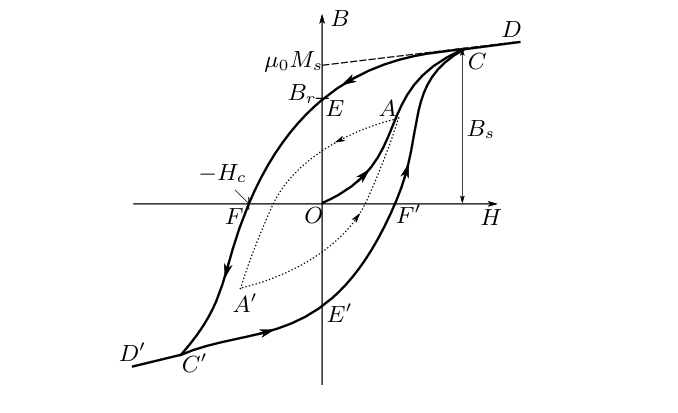
\includegraphics[width=4.5cm]{pick1.PNG}
  \caption{Теоретический вид петли гистерезиса.}
  \label{Theor}
\end{wrapfigure}

Если к ферромагнитному образцу прикладывать переменное внешнее магнитное поле, то~его состояние на плоскости $H-B$ будет изменяться по замкнутой кривой~-- \textit{петле гистерезиса}.
Резмер петли определяется максимальным значением напряжённости $H$ в цикле (например, петля $AA'$, обозначенная пунктиром на рисунке \ref{Theor}).
Если амплитуда напряжённости достаточно велика, то образец будет периодически достигать \textit{насыщения},
что на рисунке \ref{Theor} соответствует кривой $CERC'E'F'C$ (\textit{предельная петля гистерезиса}).
Пересечение предельной петли~с вертикальной осью соответствует остаточной индукции $B_r$, пересечение~с горизонтальной осью -- коэрцитивному полю $H_c$.
Крайние точки петель, соответствующие амплитудным значениям $H$ (например, точка $A$ на рисунке \ref{Theor}), лежат на \textit{начальной кривой намагничивания} ($OAC$).
\newpage

Магнитную индукцию $B$ удобно определять с~помощью ЭДС, возникающей при измерении магнитного потока $\Phi$ в катушке, намотанной на образец. Пусть катушка с $N$ витками плотно охватывает образец сечением $S$, и индукция $B$ в образце однородна. Тогда
\[\left\lvert B \right\rvert =\frac{1}{SN} \int \varepsilon  dt \]
Таким образом, для определения $B$ нужно проинтегрировать сигнал, наведённый меняющимся магнитным полем в измерительной катушке, намотанной на образец.

Для интегрирования в работе используется \textit{интегрирующая RC-цепочка}.
Входное напряжение от источника $U_{\text{вх}}(t)$ подаётся на последовательно соединённые резистор $R_{\text{и}}$ и конденсатор $C_{\text{и}}$.
Выходное напряжение $U_{\text{вых}}(t)$ снимается с~конденсатора.
Предположим, что (1) сопротивление источника мало по сравнению с~$R_{\text{и}}$;
(2) выходное сопротивление (сопротивление на входе осциллографа), напротив, велико:
$R_{\text{вых}}\gg R_{\text{и}}$; и, наконец, (3) сопротивление $R_{\text{и}}$ достаточно велико,
так что почти всё падение напряжения приходится на него, а $U_{\text{вых}}\ll U_{\text{вх}}$.
В~таком случае ток цепи равен $I=\frac{U_{\text{вх}}-U_{\text{вых}}}{R_{\text{и}}}\approx\frac{U_{\text{вх}}}{R_{\text{и}}}$,
и входное и выходное сопротивление связаны соотношением\[U_{\text{вых}}\frac{q}{C_{\text{и}}}=\frac{1}{C_{\text{и}}}\int_0^tI\text{d}t\approx\frac{1}{\tau_{\text{и}}}\int_0^tU_{\text{вх}}\text{d}t,\]где $\tau_{\text{и}}=R_{\text{и}}C_{\text{и}}$ -- постоянная времени $RC$-цепочки.
Для индукции поля получаем\[\left|B\right|=\frac{1}{SN}\int U_{\text{вх}}\text{d}t=\frac{\tau_{\text{и}}}{SN}U_{\text{вх}}.\]

Уточним, когда наше предположение справедливо. Необходимо, чтобы было выполнено \[U_\text{вых} / U_\text{вх} = \frac{\frac{1}{\omega C_\text{и}}}{\sqrt{R_\text{и}^2 + \frac{1}{\omega^2 C_\text{и}^2}}},\]
то есть $R \gg \frac{1}{\omega C}$, что равносильно $\tau_\text{и} = R_\text{и}C_\text{и} \gg \frac{1}{\omega}$ (характерное время релаксации много больше периода вынужденных колебаний).

\section{Экспериментальная установка}

Схема экспериментальной установки показана на рис. 2.
	
	Действующее значение переменного тока в обмотке N0 измеряется амперметром А (мультиметром GDM). Последовательно с амперметром включено сопротивление $R_{0}$, напряжение с которого подается на вход X электронного осциллографа (ЭО). Это напряжение пропорционально току в обмотке $N_{0}$, а следовательно и напряженности H магнитного поля в образце.
	
	Для измерения магнитной индукции B с измерительной обмотки $N_{И}$ на вход интегрирующей RC -цепочки подается напряжение $U_{И}$ (UВХ), пропорциональное производной $\dot{B}$, а с выхода снимается напряжение $U_{C}$($U_{ВЫХ}$), пропорциональное
	величине B , и подается на вход Y осциллограа.
Замкнутая кривая, возникающая на экране, воспроизводит в некотором масштабе (различном для осей X и Y ) петлю гистерезиса. Чтобы придать этой кривой количественный смысл, необходимо установить масштабы изображения, т.е. провести калибровку каналов X и Y ЭО.

\begin{figure}[h!]
	\centering
	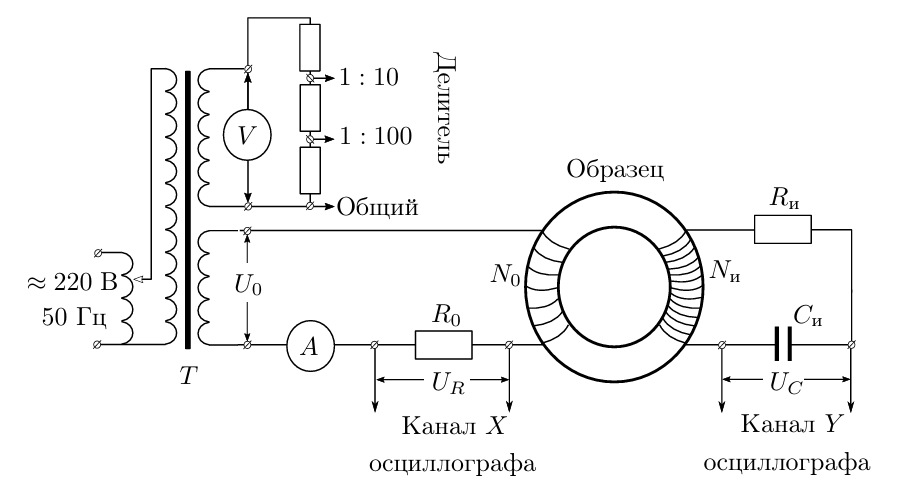
\includegraphics[width=12cm]{pick2.PNG}
	\caption{Схема установки для исследования намагничивания образцов}
	\label{fig:Holl2}
\end{figure}


\section{Обработка результатов}

\subsection{Измерение петли гистерезиса}

Подберем ток питания в намагничивающей обмотке, так чтобы была видна предельная петля гистерезиса. Затем уменьшим ток до исчезновения усов.\par
Подберем коэффициенты усиленияя для улучшения картинки на осциллографе. Далее зарисуем и сфотографируем предельную петлю(рис.3 и рис.4)


\begin{figure}[htbp]
    \centering 
    
    \begin{subfigure}[b]{0.3\textwidth} 
        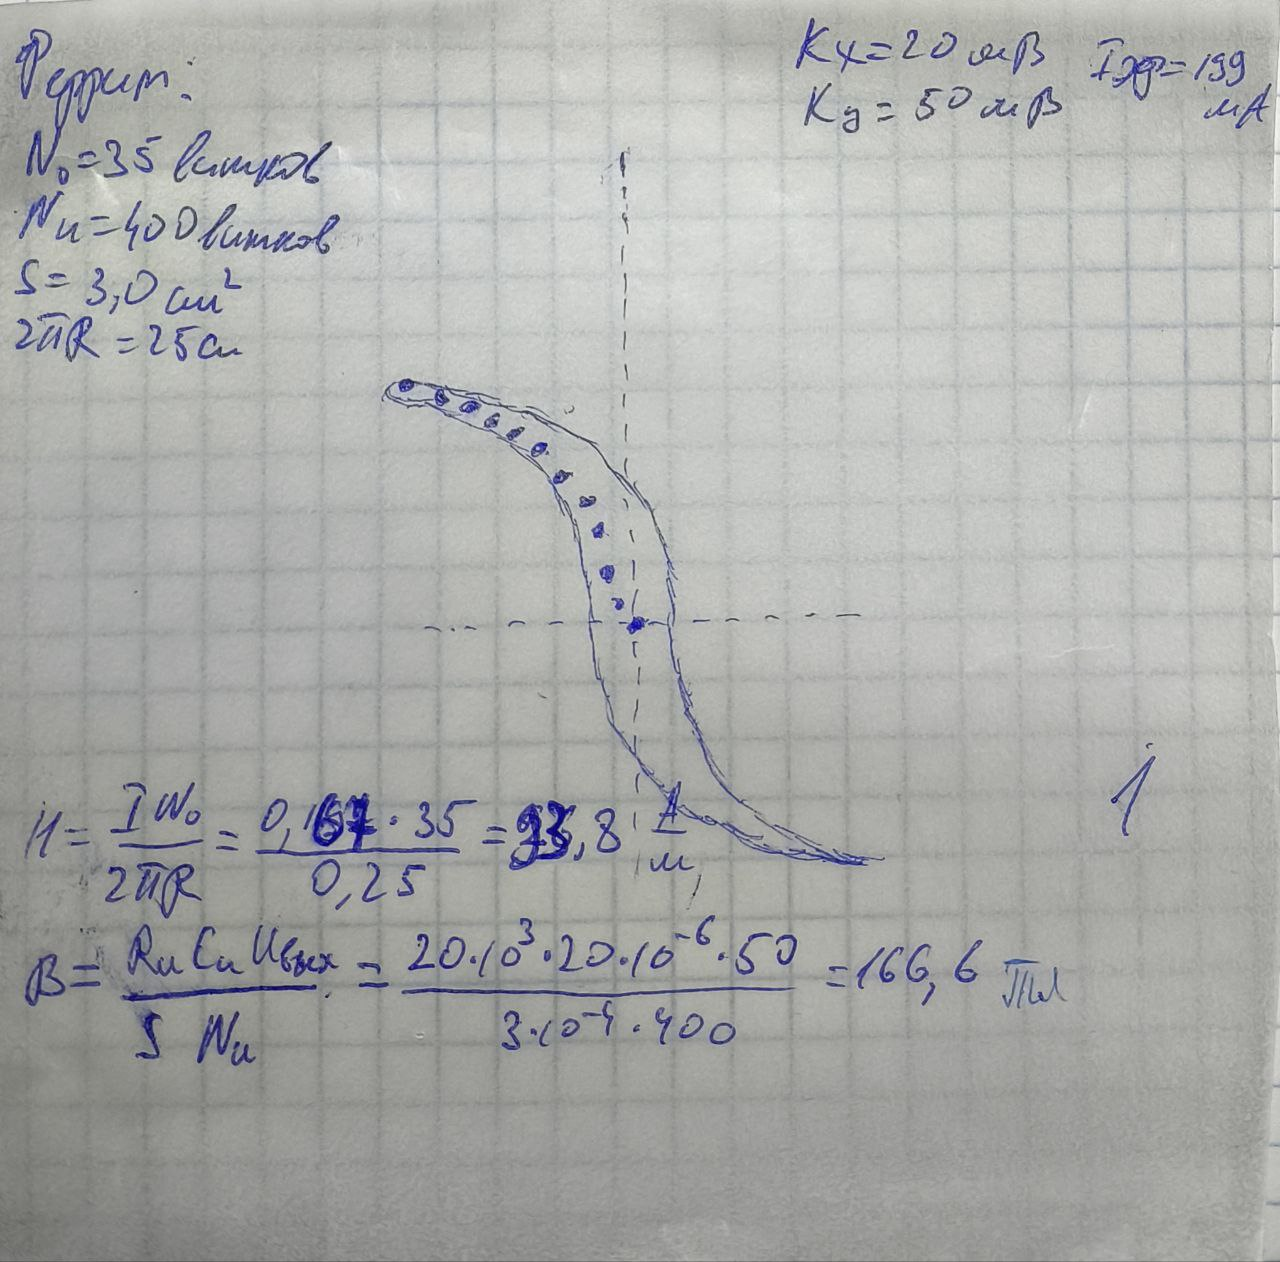
\includegraphics[width=\linewidth]{p1.jpg} 
        \caption{Феррит} 
        \label{fig:image1}
    \end{subfigure}
\hfill 
\begin{subfigure}[b]{0.3\textwidth}
    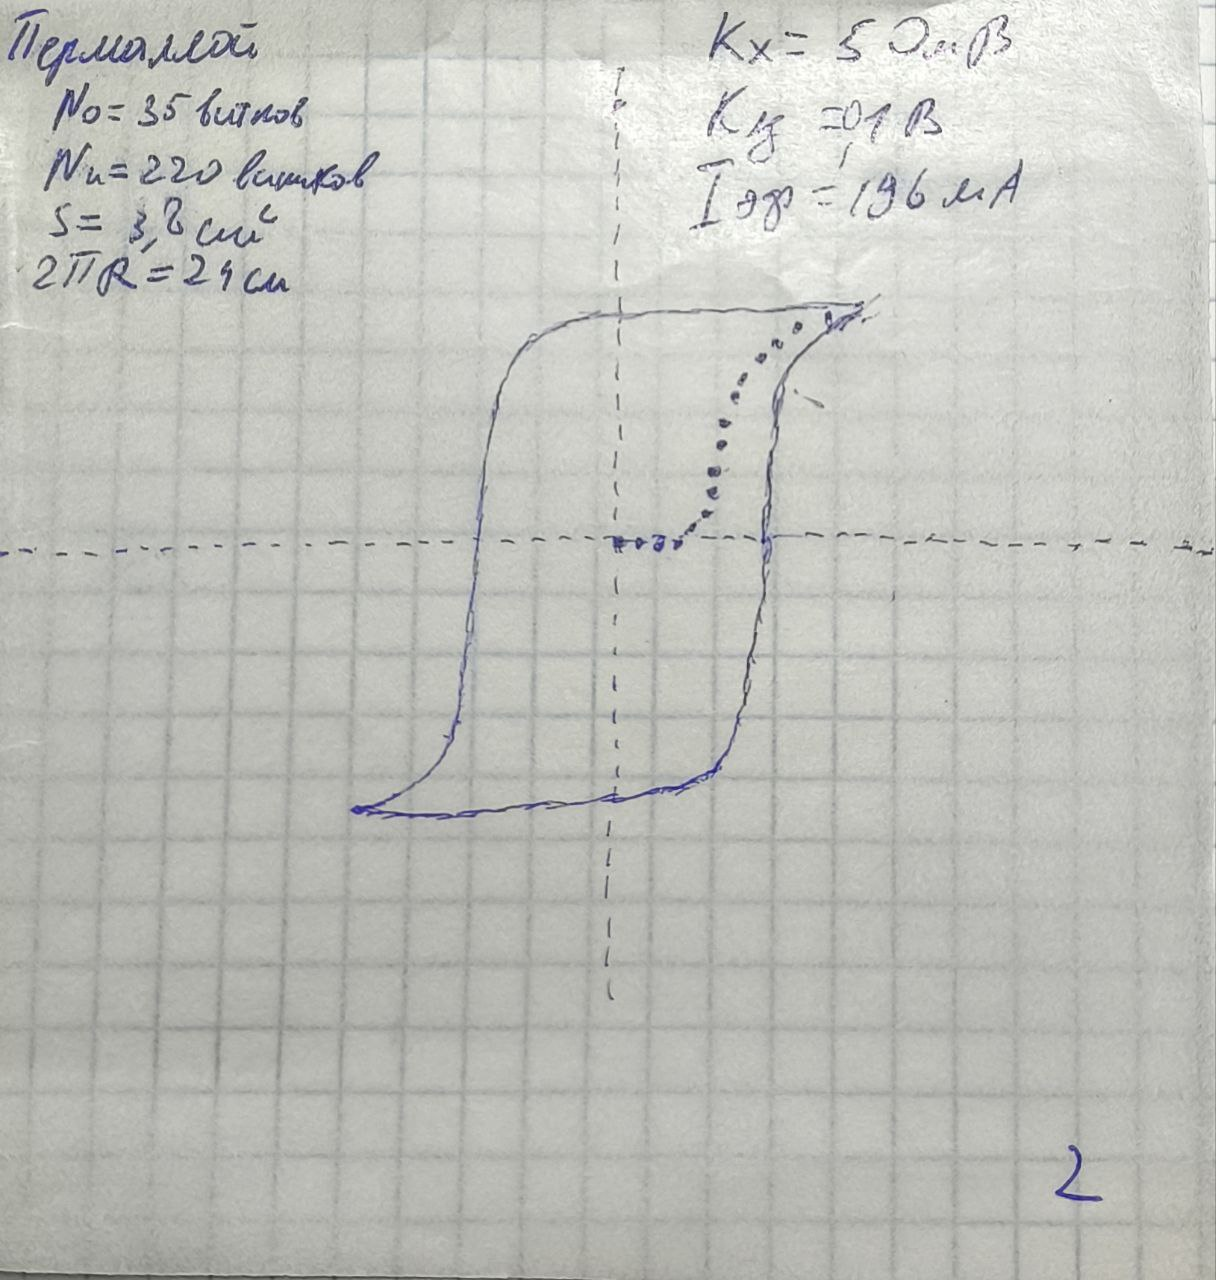
\includegraphics[width=\linewidth]{p2.jpg}
    \caption{Пермаллой} 
    \label{fig:image2}
\end{subfigure}
\hfill
\begin{subfigure}[b]{0.3\textwidth}
    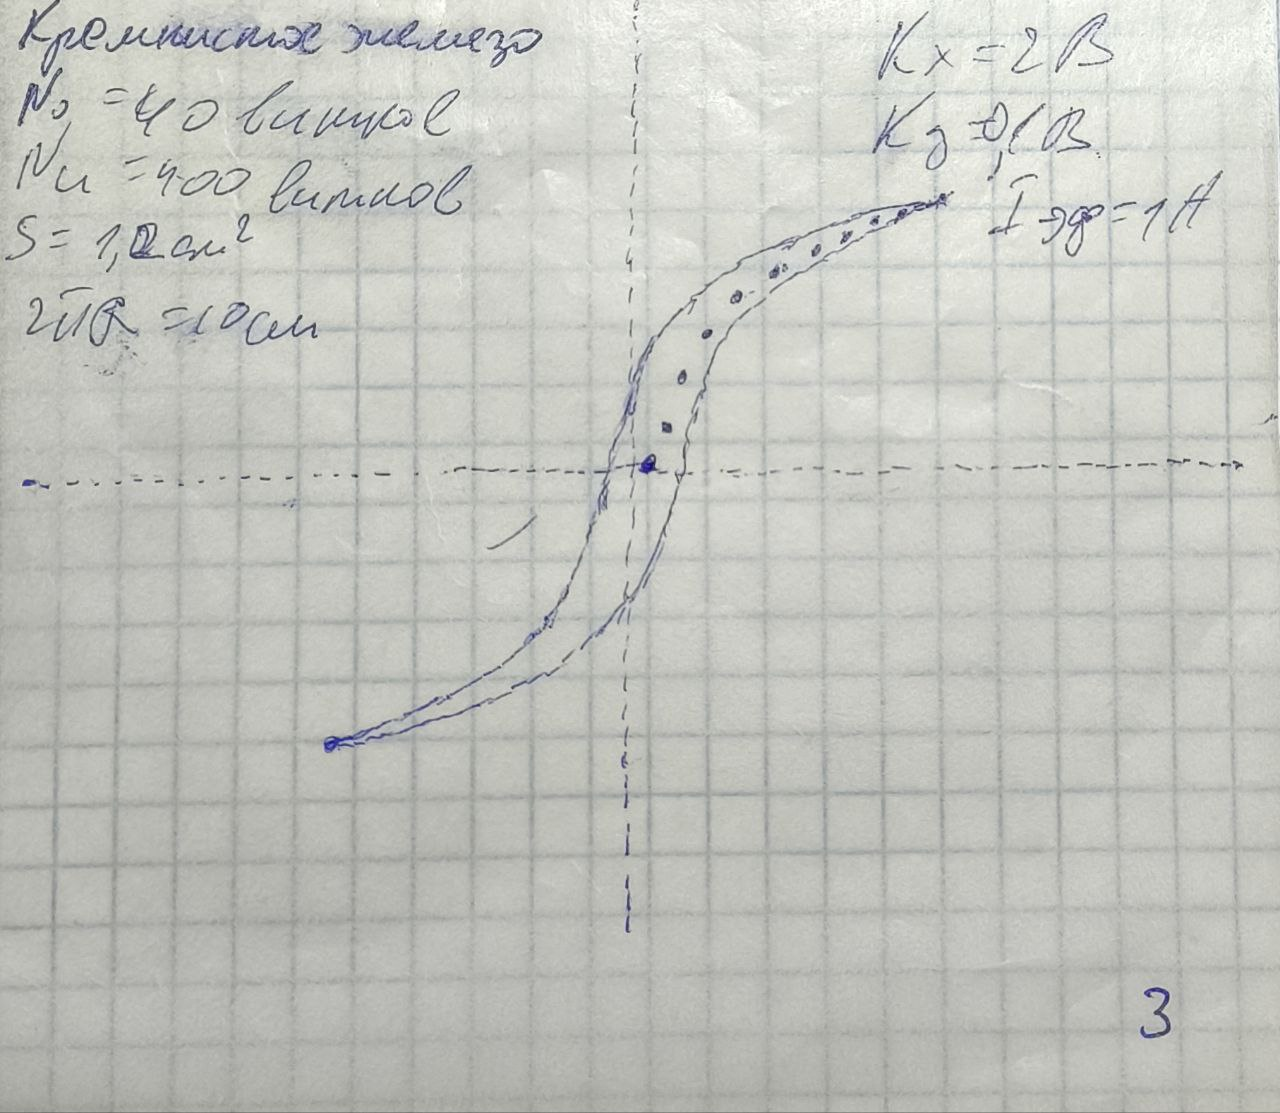
\includegraphics[width=\linewidth]{p3.jpg}
    \caption{Кремниевое железо} 
    \label{fig:image3}
\end{subfigure}
    
\caption{Рисунки на кальке} 
\label{fig:three_images}

\end{figure}




\begin{figure}[htbp]
    \centering 
    
    \begin{subfigure}[b]{0.3\textwidth} 
        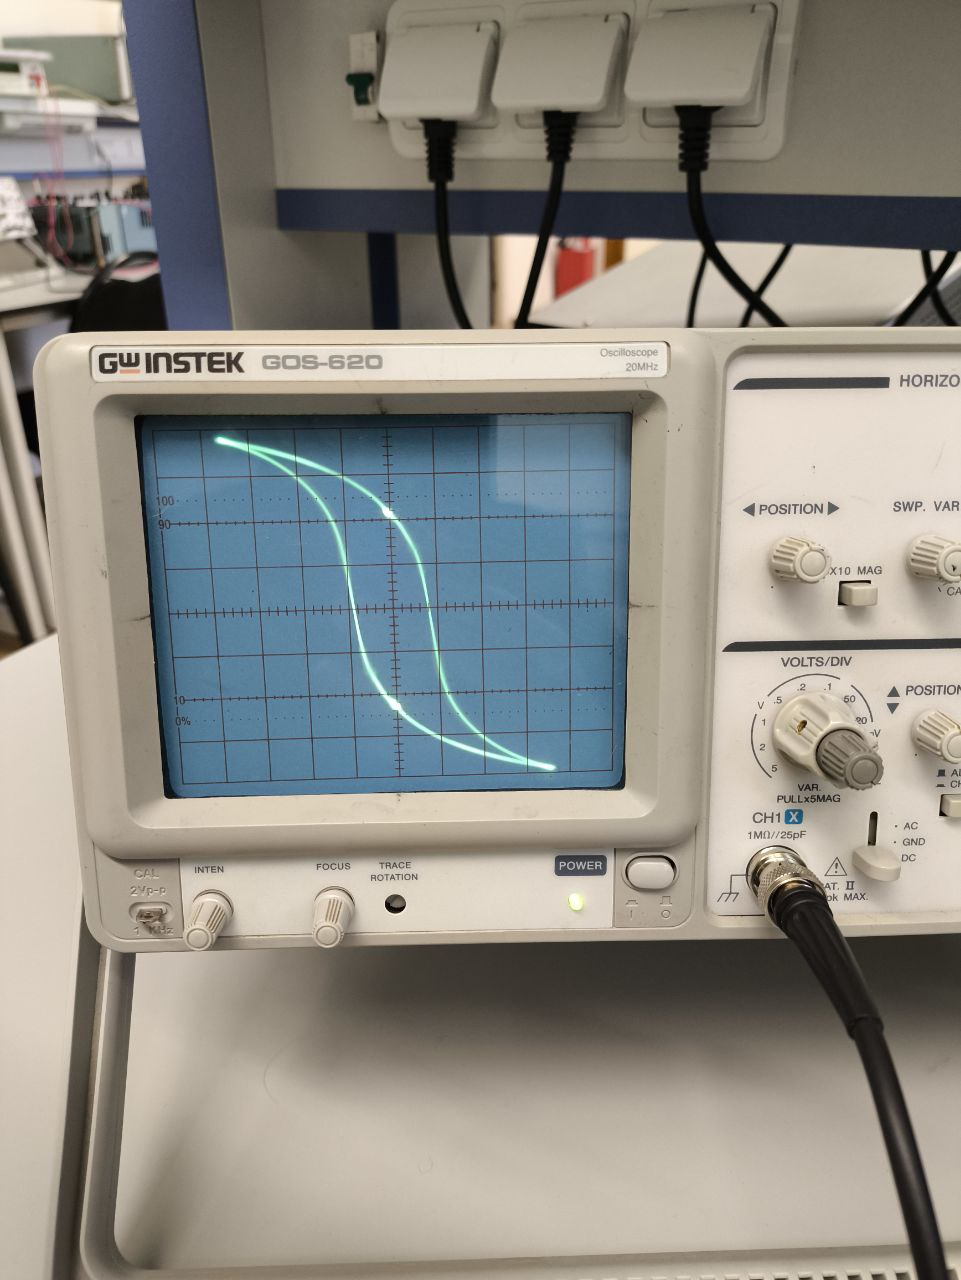
\includegraphics[width=\linewidth]{p5.jpg} 
        \caption{Феррит} 
        \label{fig:image1}
    \end{subfigure}
\hfill 
\begin{subfigure}[b]{0.3\textwidth}
    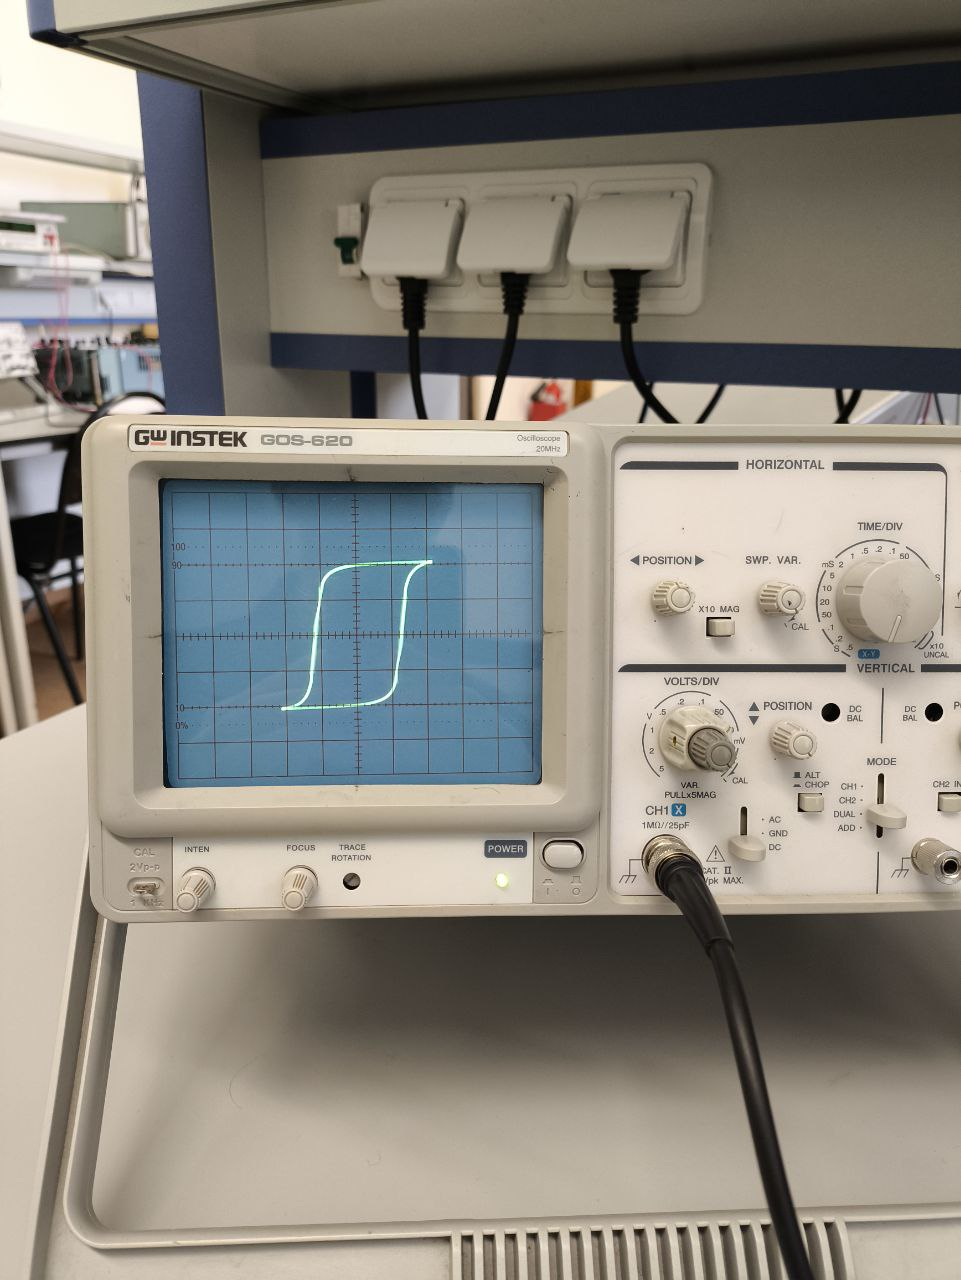
\includegraphics[width=\linewidth]{p4.jpg}
    \caption{Пермаллой} 
    \label{fig:image2}
\end{subfigure}
\hfill
\begin{subfigure}[b]{0.3\textwidth}
    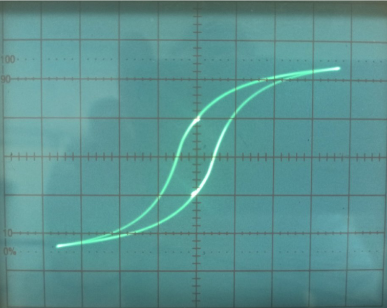
\includegraphics[width=\linewidth]{p6.PNG}
    \caption{Кремниевое железо} 
    \label{fig:image3}
\end{subfigure}
    
\caption{Фотографии с осциллографа} 
\label{fig:three_images}

\end{figure}




Измерим полную ширину и высоту предельной петли $(2X_{s} и 2Y_{s})$, 
соответствующие удвоенной амплитуде колебаний напряженности $H_{s}$ и индукции $B_{s}$




\begin{tabular}{|c|c|c|c|} 
    \hline 
    &Феррит & Пермаллой & Кремниевое железо \\
    \hline 
    $2X_{s}$ & 20 дел & 22 дел & 26 дел \\
    \hline
    $2Y_{s}$  & 20 дел  & 22 дел  & 8 дел  \\
    \hline
\end{tabular}

Измерим двойные амлитуды для коэртитивного поля $2X_{c}$ и остаточной индукции $2Y_{r}$


\begin{tabular}{|c|c|c|c|} 
    \hline 
    &Феррит & Пермаллой & Кремниевое железо \\
    \hline 
    $2X_{c}$ & 4 дел & 12 дел & 3 дел \\
    \hline
    $2Y_{r}$  & 6 дел  & 20 дел  & 8 дел  \\
    \hline
\end{tabular}

\newpage

Рассчитаем цену деления шкалы ЭО для петли в $\frac{\text{А}}{\text{м}}$ для Феррита и для других материалов:

\[H = \frac{IN_{0}}{2\pi  R} = \frac{0,67*35}{0,25} = 9,3 \pm 0,9 \frac{\text{А}}{\text{м*дел}}\]

\[B = \frac{R_{\text{и}}C_{\text{и}}U_{\text{вых}}}{S N_{\text{и}}} = \frac{20*10^{3}*20*10^{-6}*50}{3*10^{-4}*400}=0,167 \pm 0,2 \frac{\text{Тл}}{\text{дел}}\]

\begin{itemize}
    \item Кремниевое железо:
    \[
    H = 90,9 \pm 0,9 \frac{\text{A}}{\text{м}}, \quad B = 0,20 \pm 0,2 \frac{\text{Тл}}{\text{дел}}\]

    
    \item Пермаллой:
    \[
    H = 10,6 \pm 0,9 \frac{\text{A}}{\text{м}}, \quad B = 1,01 \pm 0,2 \frac{\text{Тл}}{\text{дел}}\]

\end{itemize}

\subsection{Проверка калибровки осциллографа}

Проведем калибровку горизонтальной оси. Закоротим обмотку и с помощью автотрансформатора подберем ток, чтобы горизонтальная прямая занимала 
большую часть.\par
Рассчитаем чувствительность канала X и сравним с выбранным коэффициентом $K_{x}$:

\[K_{x} = \frac{2R_{0} \sqrt{2} I_{\text{эф}}}{2x} = 17,0 \pm 0,1 \frac{\text{мВ}}{\text{дел}} (\text{для феррита})\]
\[K_{x} = \frac{2R_{0} \sqrt{2} I_{\text{эф}}}{2x} = 46,0 \pm 0,1 \frac{\text{мВ}}{\text{дел}} (\text{для пермаллоя})\]
\[K_{x} = \frac{2R_{0} \sqrt{2} I_{\text{эф}}}{2x} = 21,1 \pm 0,1 \frac{\text{В}}{\text{дел}} (\text{для кремнистого железа})\]

Для проверки калибровки оси Y соединим вход Y осциллографа с клеммами делителя 1/100 и общий\par
Подберем коэффициент $K_{y}$ с помощью трансформатора и далее с помощью мультиметра найдем величину $U_{\text{эфф}}$.Далее по формуле рассчитаем чувствительность:

\[K_{y1} = \frac{2 \sqrt{2} U_{\text{эфф}}}{2y} = \frac{2 \sqrt{2}*0,027}{6,4} = 35,3 \pm 0,1 \frac{\text{мВ}}{\text{дел}}\]

\[K_{y2} = \frac{2 \sqrt{2} U_{\text{эфф}}}{2y} = \frac{2 \sqrt{2}*0,155}{5,4} = 81,1 \pm 0,1 \frac{\text{мВ}}{\text{дел}}\]

\[K_{y3} = \frac{2 \sqrt{2} U_{\text{эфф}}}{2y} = \frac{2 \sqrt{2}*0,151}{5,8} = 73,2 \pm 0,1 \frac{\text{мВ}}{\text{дел}}\]

\subsection{Определение $\tau$ - постоянной времени интегрирующей ячейки}

Отключим канал X и подберем напряжение, чтобы прямая занимала большую часть экрана. Далее по формуле найдем входное напряжение:
\[U_{\text{вх}} = 2y*K_{y} = 6,8*2 = 13,6 \pm 0,2 \text{В}\]

Не меняя тока, соединим Y с выходом ячейки и найдем аналогичным образом $U_{\text{вых}}$:
\[U_{\text{вых}} = 2y*K_{y} = 6,8*20*10^{-3} = 0,108 \pm 0,201 \text{В}\]
Рассчитаем $\tau$:
\[\tau = \frac{U_{\text{вх}}}{\omega *U_{\text{вых}} } = \frac{13,6}{0,108*6,28*50} = 0,401 \pm 0,012 \text{с}\]
\[\tau_{RC} = R_{\text{и}}*C_{\text{и}}=0,4 \text{с}\]


\begin{table}[h]
\centering
\begin{tabular}{|c|c|c|c|}
\hline
Ампл. & Термаллой & Fe-Si & Феррит \\
\hline
\( H_{max}, \frac{A}{M} \) & 0,20 $\pm 0,03$ & 2,4 $\pm 0,8$ & 0,186 $\pm 0,031$\\
\hline
\( H_{c}, \frac{A}{M} \) &0,12 $\pm 0,07$  &0,27 $\pm 0,28$ &0,0186 $\pm 0,0014$ \\
\hline
\( B_r, T \) &0,020$\pm 0,005$ & $0,005 $$\pm 0,001$  &0,0001 $\pm 0,0043$ \\
\hline
\( B_s, T \) &0,020$\pm 0,008$ &0,002$\pm 0,001$  &0,003 $\pm 0,001$ \\
\hline
\( \mu_{\text{пач}} \) &0,10$\pm 0,05$ &2,50 $\pm 0,05$ &3,80 $\pm 0,05$\\
\hline
\( \mu_{\text{max}} \) &3,30 $\pm 0,05$ &2,90 $\pm 0,05$ & 4,00 $\pm 0,05$\\
\hline
\end{tabular}
\caption{Параметры магнитных материалов}
\label{tab:magnetic_params}
\end{table}


\textbf{Вывод} \par

Изучил петлю гистерезиса различных ферромагнитных материалов в переменных полях. Проверил теоретические значения со значениями,
полученными на практике. Произвел работу с осциллографом и мультиметром для снятия значений. Сделал все необходимые рассчеты и записал их.

\end{document}